\section{Design/Approach/Methodology} 



\label{sec:design}

This section describes the methodology we employed from scratch to overcome the challenges in distinguishing between gaming and music video traffic on YouTube. We designed an approach that incorporates data collection, feature extraction, and model training to achieve accurate and adaptive classification.

\vspace{2mm}


The implemented pipeline works as follows :
\begin{itemize}
    \item \textbf{Data Collection:} The first step in our methodology involves capturing network traffic data directly from Youtube, we aim to collect traffic traces from both gaming and music video. In order to do so, and to ensure sufficient diversity within our dataset, we collected approximately 2000 seconds of data by recording 18 videos for training and 2 videos for testing, each with 100 seconds of traffic data. This process resulted in around 15,000 rows of data for analysis.
    \item \textbf{Traffic Capture:} We log raw network traffic into two\texttt{.pcap} files respectively for the two categories we are trying to distinguish, as the pipeline is streaming the videos. This captures essential data such as packet size and frequency or any other data that would be useful to help our model labeling videos.
    \item \textbf{Feature Extraction:} Once the \texttt{.pcap} files are generated, they are converted into \texttt{.csv} files.
    \item \textbf{Data Upload:} After feature extraction and conversion, we upload the resulting files to a designated server for storage and analysis. This ensures all processed data is centrally accessible for model training.
    \item \textbf{Traffic Management:} The pipeline is designed to manage resource limits well so that the data collection processes work well without over-overloading the system.
\end{itemize}


The following features come from the packet traces and are used as input for our machine learning models,They provide important information on the unique traffic patterns of gaming and music videos, which helps us classify them accurately :
\begin{itemize}
    \item \textbf{Packet Size:} Measures the size of each packet transmitted.
    \item \textbf{Packet Frequency:} Tracks how often packets are sent during the transmission.
    \item \textbf{Data Spikes:} Observes fluctuations in upload/download rates.
\end{itemize}

\begin{figure}[ht]
    \centering
    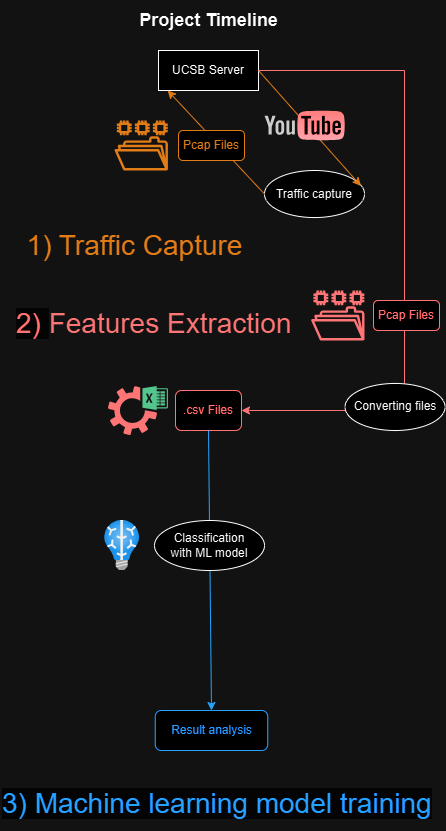
\includegraphics[width=1.0\linewidth]{timeline_diagram.png}
    \label{fig:your_label}
\end{figure}


Regarding our Machine Learning model, we use a Random Forest model for our classification task. This algorithm processes the input data (that we have previously stored in our .csv files) through an ensemble of decision trees, where each tree and sub-tree analyze and compare different given features, contributing to the final prediction. By combining the outputs of multiple trees, the model generates classifications based on the patterns it has learned during training.

\vspace{2mm}

The design of our methodology is guided by the following principles:
\begin{itemize}
    \item \textbf{Custom Dataset:} By focusing on YouTube traffic and manually selecting videos, we ensure the dataset align with the targeted problem.
    \item \textbf{Feature Relevance:} The selected features capture the nuances of gaming and music video traffic.
    \item \textbf{Small-Scale Feasibility:} The amount of readily available content on YouTube  makes this project achievable while sticking with a small-scale framework.
    \item \textbf{Use of Machine Learning:} Machine learning techniques allow us to overcome the challenges posed by traditional classification approaches and provide flexible solutions for evolving applications.
\end{itemize}

This approach provides a strong starting point for and gives us the opportunity to explore and improve further the network traffic classification.


